Цель:
\begin{enumerate}
  \item Написание графического интерфейса пользователя для системы coex. В графическом интерфейсе необходимо предусмотреть выбор директорий для работы системы и вывод информации
  \item Адаптировать плагин Media scanner
\end{enumerate} 

Для создания интерфейса использовался Qt Designer — кроссплатформенная свободная среда для разработки графических интерфейсов (GUI) программ, использующих библиотеку Qt. Входит в состав Qt framework. При разработке использовался подход сигналов и слотов. Сигналы и слоты --- подход, который позволяет реализовать шаблон <<наблюдатель>>, минимизируя написание повторяющегося кода. Концепция заключается в том, что компонент может посылать сигналы, содержащие информацию о событии. В свою очередь другие компоненты могут принимать эти сигналы посредством специальных функций — слотов. Данный подход был выбран потому что он хорошо подходит для описания графического интерфейса пользователя.
Так как система coex является консольной утилитой, то графический интерфейс генерирует строку с необходимыми параметрами и запускает с ними консольную утилиту, перехватывая вывод и отображая его в интерфейсе. В качестве параметров выступают директории для работы системы. Главное окно представлено на рисунке~\ref{ship_1:ship_1}.

\begin{figure}[h!]
\center{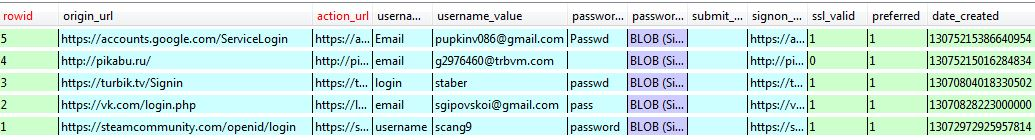
\includegraphics[width=0.5\linewidth]{ship_1}}
\caption{Главное окно}
\label{ship_1:ship_1}
\end{figure}

Интерфейс состоит из следующих элементов:
\begin{enumerate}
  \item Кнопка <<Открыть папку>> отвечает за выбор папки, в которой будет производиться поиск
  \item Кнопка <<Сохранить в папку>> отвечает за выбор папки для сохранения результатов
  \item В данном окне отображается вывод процесса выполнения.
  \item Кнопка <<Запуск>> отвечает за запуск системы.s
  \item Окно, в котором находятся текущие плагины для выполнения в виде списка.
Если не выбраны директории для работы, то при нажатии на кнопку <<Запуск>> отобразиться соответствующее сообщение (рисунок 2). Диалоговое окно выбора директории представлено на рисунке 3. Процесс выполнения системы представлен на рисунке 4. По завершению работы системы отобразиться соответствующие сообщение (рисунок 5).
\end{enumerate}

рисунке~\ref{ship_2:ship_2}
рисунке~\ref{ship_3:ship_3}
рисунке~\ref{ship_4:ship_4}
рисунке~\ref{ship_5:ship_5}

\begin{figure}[h!]
\center{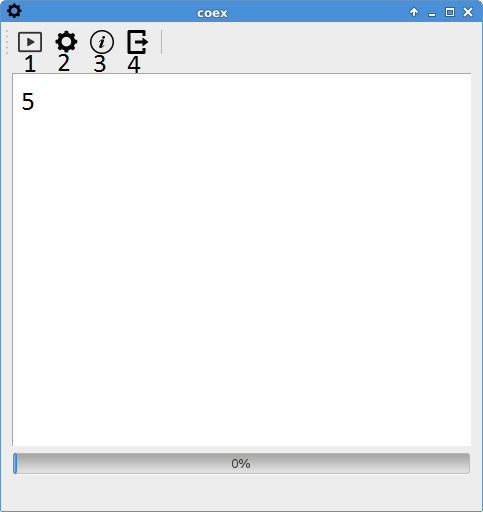
\includegraphics[width=0.5\linewidth]{ship_2}}
\caption{ Ошибка }
\label{ship_2:ship_2}
\end{figure}

\begin{figure}[h!]
\center{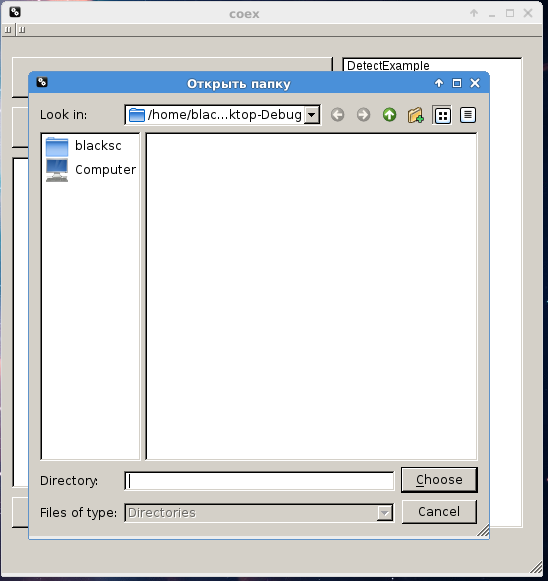
\includegraphics[width=0.5\linewidth]{ship_3}}
\caption{ Выбор директории }
\label{ship_3:ship_3}
\end{figure}

\begin{figure}[h!]
\center{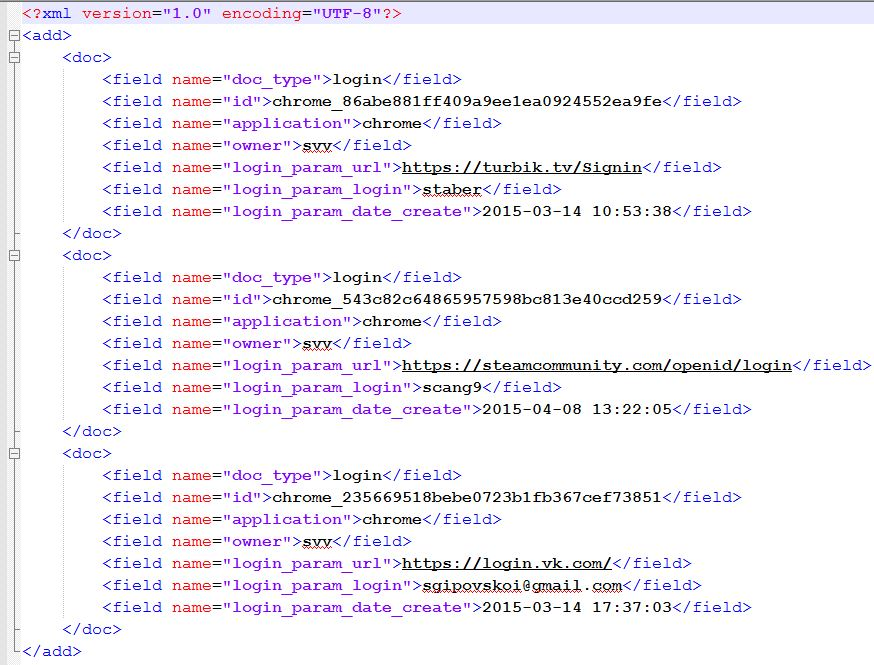
\includegraphics[width=0.5\linewidth]{ship_4}}
\caption{ Процесс выполнения }
\label{ship_4:ship_4}
\end{figure}

\begin{figure}[h!]
\center{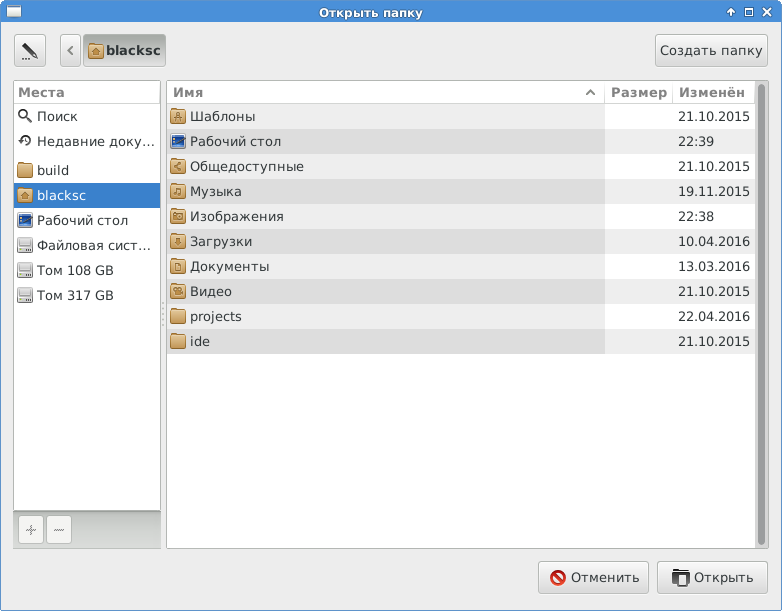
\includegraphics[width=0.5\linewidth]{ship_5}}
\caption{ Сообщение о выполнении }
\label{ship_5:ship_5}
\end{figure}


Программный модуль media scanner осуществляет нахождение медиа-файлов (аудио, видео, изображение) и извлечение мета-данных с записью их в XML формат. Данный программный модуль не соответствовал следующим условиям при которых система распознает его как плагин:
\begin{enumerate}
  \item 
  \item директория для временных файлов /tmp;
  \item исходный код должен находится в папке /src;
  \item *.pro файл должен именоваться Task*.pro;
  \item файлы *.cpp и *.h должны соответствовать шаблону TaskExample;
\end{enumerate}

После выполения данных условий система coex успешно распознает,собирает (рисунок 6) и выполняет данный плагин (рисунок 7). Результаты выполнения представлен на рисунке 8.


рисунке~\ref{ship_6:ship_6}
рисунке~\ref{ship_7:ship_7}
рисунке~\ref{ship_8:ship_8}

\begin{figure}[h!]
\center{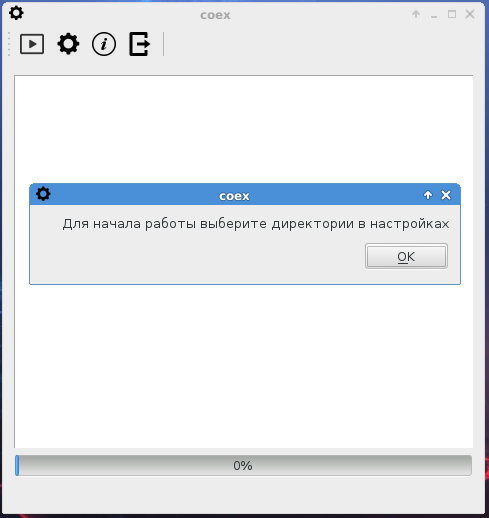
\includegraphics[width=0.5\linewidth]{ship_6}}
\caption{ Успешная сборка плагина }
\label{ship_6:ship_6}
\end{figure}

\begin{figure}[h!]
\center{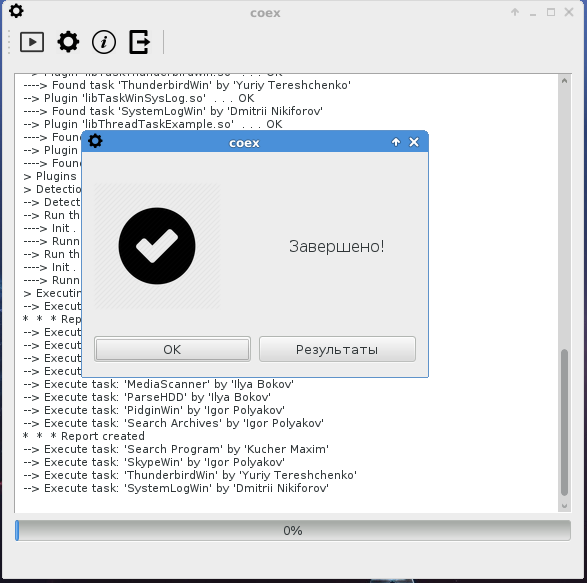
\includegraphics[width=0.7\linewidth]{ship_7}}
\caption{ Выполнение плагина }
\label{ship_7:ship_7}
\end{figure}

\begin{figure}[h!]
\center{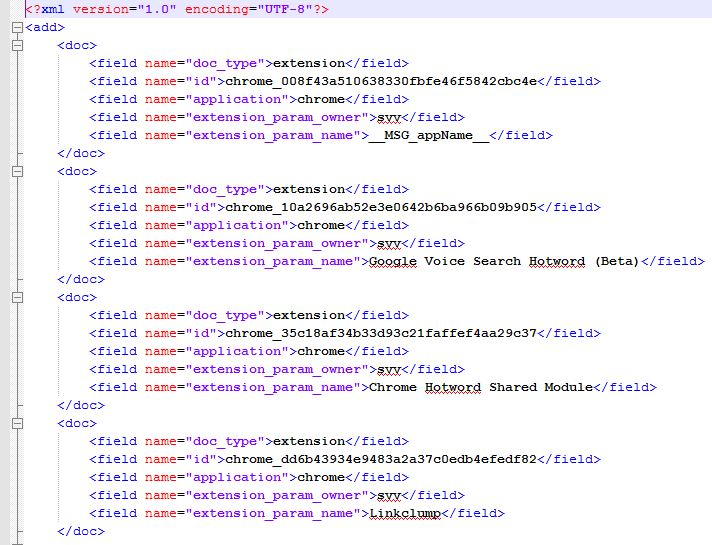
\includegraphics[width=0.9\linewidth]{ship_8}}
\caption{ Результат выполнения плагина }
\label{ship_8:ship_8}
\end{figure}

\clearpage










